\documentclass{polytech/polytech}
      
\usepackage{lipsum}
  
\typereport{prddi5}       

\reportyear{2015-2016}   

\title{Exemple d'utilisation de la classe de document \mbox{polytech}}
\subtitle{Il peut y avoir un sous titre mais ce n'est pas obligatoire}
\reportlogo{polytech/polytech}
           
\student[di5]{Pierre}{Premier}{pierre.premier@example.com}
\student[di4]{Paul}{Deuxième}{paul2@example.com}
\student[none]{Paul}{Deuxième}{paul2@example.com}
\student{Jacques}{Un peu plus Long}{j.unpeupluslong@example.com}

\academicsupervisor[di]{First}{Supervisor}{first.supervisor@example.com}
\academicsupervisor[dee]{Second}{Supervisor}{second.supervisor@example.com}
\academicsupervisor{Machin}{Chose}{machin.chose@example.com}

\industrialsupervisor[Fonction très importante]{Un}{Gars}{un.gars@example.com}
\industrialsupervisor{Un deuxième}{Gars}{undeuxieme.gars@example.com}

\company[polytech/polytech]{La grosse compagnie}{1 rue de l'étrange\\999999 Dans vos rèves}{example.com}

\confidential

\resume{\lipsum[1]}
\motcle{mot}
\motcle{clé}            
\motcle{deux mots}
             
\abstract{\lipsum[1-2]}
\keyword{word}
\keyword{key}
\keyword{two words}
\keyword{fourth word}


\posterblock{Objectifs}{
Lorem ipsum dolor sit amet:
\begin{itemize}
\item Vestibulum tincidunt ipsum
\item In dictum elit condimentum.
\item Suspendisse ornare orci.
\end{itemize}
Aliquam porta mi ut justo pellentesque porta.
}{polytech/polytech}{dictum elit condimentum}

\posterblock{Mise en \oe{}uvre}{
Mauris consectetur, et auctor mi \emph{fermentum}.  Etiam venenatis augue neque, ac ullamcorper sodales sit amet.
\begin{center}
\begin{tabular}{|c|c|c||c|}
\hline
1&2&3&4\\
\hline
\end{tabular}
\end{center}
Fusce aliquet sed sapien \textbf{tempor} facilisis. Nunc mi urna, cursus a ullamcorper quis, laoreet id felis.  
}{polytech/polytech}{}%Encore le logo au cas où on ne l'aurait pas vu}

\posterblock{Résultats attendus}{
\begin{itemize}
\item Quisque \textbf{dictum} diam in feugiat
\item Proin quam nec, gravida mi
\item \textbf{\emph{Suspendisse} truc bidul} vehicula magna
\item Nulla sagittis diam congue sagittis
\item Donec auctor a non nisi
\item Vestibulum quis \emph{rhoncus} risus
\end{itemize}%
}{polytech/polytech}{auctor a non nisi\\auctor a non nisi}
    
\bibliography{biblio}

\begin{document}

\chapter{Test includepdf}

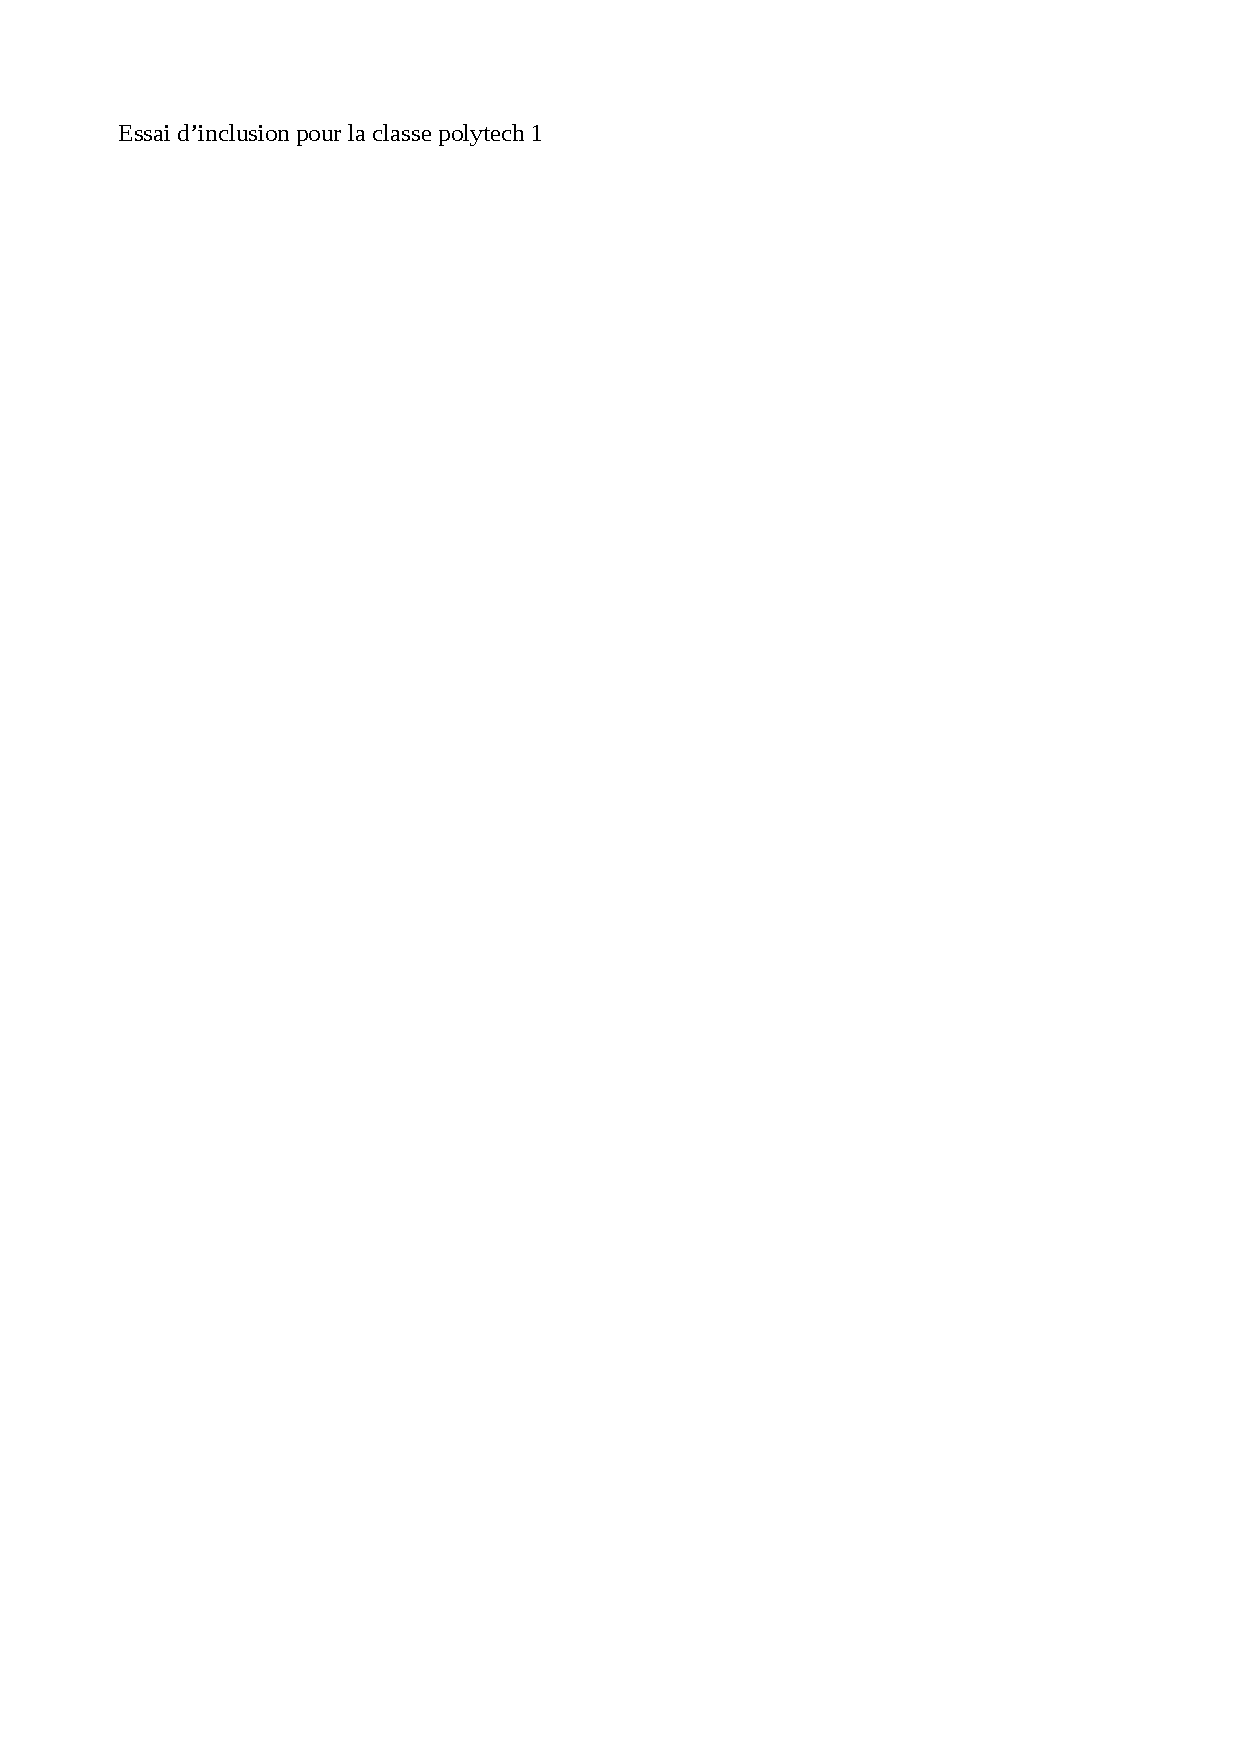
\includepdf[pages=-,templatesize={\textwidth}{\textheight}]{includeme.pdf}            

             
\chapter*[Titre court pour l'entête]{Introduction générale du rapport avec un titre un peu long}

\lipsum[1-5]
\section{Ma section}

\lipsum[1-3]

\subsection{Ma section}

\lipsum[1-3]

\subsubsection{Ma section}

\lipsum[1-3]

\paragraph{Ma section}

\lipsum[1-3]

\subparagraph{Ma section}

\lipsum[1-3]

\section{Une section n'est jamais seule, donc j'en ajoute au moins une autre et le titre peut être long si nécessaire}

\lipsum[1-3]
                       
\section{Le dicton dit \og{}Jamais deux sans trois\fg{}, donc j'en ajoute au moins une autre et le titre peut être long si nécessaire mais il ne faut pas abuser car ça devient moche et peu explicite sinon}

\lipsum[1-3] 

\part{Les premiers trucs dont je vais parler}                

\chapter{Le tout premier truc}   

\lipsum[1]
           
\section{Pour ne pas se casser la tête}

\lipsum[1-6]

\part{essai}
 
\chapter{essai:chap1}
      
\lipsum[1-4]
     
\section{truc}

\chapter*{essai:chap2}
     
\lipsum[1-4]

\section{truc}

  
\chapter{truc}
\lipsum[1-20]         
 
\section{Ma section}
\lipsum[1-5]

\section{Ma section}
\lipsum[1-5]

          
\subsection{Ma section}
\lipsum[1-5]
\subsection{Ma section}
\lipsum[1-5]
\subsubsection{Ma section}
\lipsum[1-5]
\subsubsection{Ma section}
\lipsum[1-5]
\paragraph{Ma section}
\lipsum[1-5]
\paragraph{Ma section}
\lipsum[1-5]
\subparagraph{Ma section}
\lipsum[1-5]
\subparagraph{Ma section}
\lipsum[1-5]
  
\chapter*{Conclusion}

\lipsum[1-2]

\appendix   

\chapter{Ma première annexe}

\lipsum[1-4]

\section{truc}

\lipsum[1-4]
 
\chapter{Ma deuxième annexe}
  

\section{truc}

\lipsum[1-4]

\end{document}


